\chapter{Single User Interaktion}
\label{ch:Single_User_Interaktion}

\section{Realisierung}

\subsection{Highlight}
\label{ch:highlight_realisierung}
Dank der Beispiel Szene im Steam-VR Asset, beschrieben im Kapitel \ref{ch:highlight}, war sehr schnell klar, wie das Highlight der Objekte bei im Asset selbst gemacht wird. \\
Um die Silhouette des Objektes gelb umrahmen zu können, wird das Material aller MeshRenderer (in Unity zuständig für die visuelle Darstellung eines GameObjects) des Objektes ersetzt, mit einem Material, auf welchem sich ein spezifischer Shader befindet. Dieser Shader zeichnet nur die Aussenlinie des Meshes und macht alles innerhalb dieser Linie transparent. Um die originale Farbe des Objektes nicht zu verlieren, wird das Objekt erst kopiert und anschliessend das Material auf dem kopierten Objekt geändert. \\

\noindent Das Highlight in der Single-User Applikation wurde genau wie im vorherigen Abschnitt beschrieben implementiert. An dein beiden Controllern des Benutzers wurde jeweils ein Collider hinzugefügt, welcher aber keine Kollision verursacht sondern lediglich ein Event feuert, sobald er mit einem anderen Collider in Berührung kommt. Diese Art der Collider wird auch Trigger genannt. \\
Dieses Event wird von der Applikation abgefangen und löst das Highlight des kollidierten Objektes aus, wie in Abbildung \ref{fig:highlight_single_user_application} zu sehen ist.

\begin{figure}[h!]
	\centering
	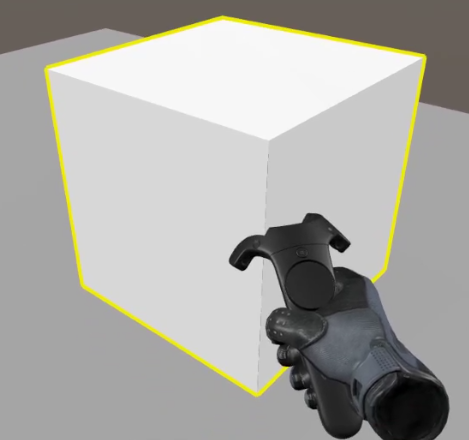
\includegraphics[keepaspectratio,width=0.4\linewidth]{img/Single_User_Highlight.PNG}
	\caption{Highlight in der Single User Applikation}
	\label{fig:highlight_single_user_application}
\end{figure}

\subsection{Snapping}
Zwischen den Bauteilen, bei welchen das Snapping stattfinden soll, wurden Trigger angebracht, welche genau aufeinander passen.(Abbildung \ref{fig:trigger_between_objects}) Sobald sich diese Trigger berühren wird ein Event ausgelöst, welches das Bauteil in der Hand des Benutzers als Silhouette am vorgesehenen Ort zeichnet. \\
Dafür wird eine Kopie des Bauteils mitsamt dem Trigger erstellt, so positioniert, dass die beiden Trigger übereinstimmen und anschliessend das Material durch den Highlight-Shader ersetzt (beschrieben in Kapitel \ref{ch:highlight_realisierung}).

\begin{figure}[h!]
	\centering
	\begin{minipage}[b]{0.49\linewidth}
		\centering
		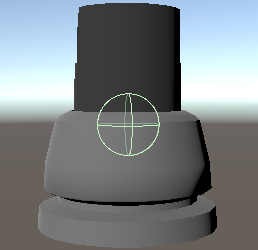
\includegraphics[keepaspectratio,width=0.9\linewidth]{img/Trigger_Between_Objects.PNG}
		\caption{Trigger zwischen Bauteilen}
		\label{fig:trigger_between_objects}
	\end{minipage}
	\hfill
	\begin{minipage}[b]{0.49\linewidth}
		\centering
		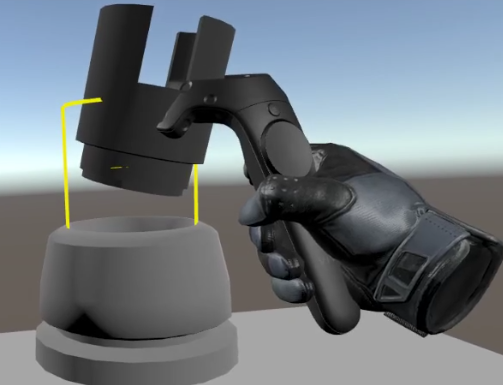
\includegraphics[keepaspectratio,width=0.9\linewidth]{img/Snapping.PNG}
		\caption{Highlight des Snappings}
		\label{fig:snapping}
	\end{minipage}
\end{figure}

\subsection{Kollision}
Um die Kollision der Bauteile so natürlich wie möglich zu machen, mussten den Bauteilen ein Rigidbody angehängt werden. Dieser ist für die Physik-Berechnungen zuständig und kann konstante Beschleunigungen oder eine konstante Geschwindigkeit auf das Bauteil geben.

% TODO: Bild referenzieren

\begin{figure}[h!]
	\centering
	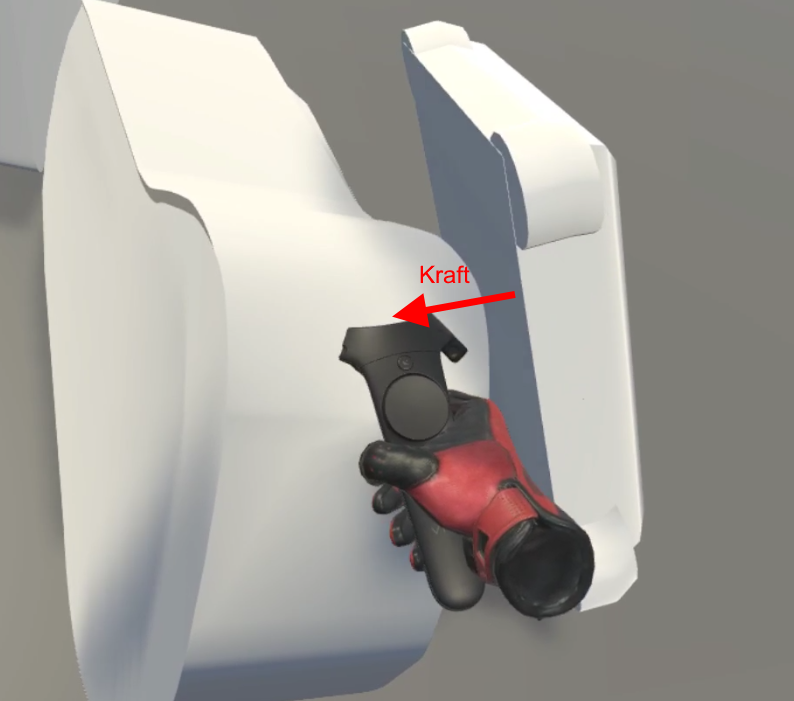
\includegraphics[keepaspectratio,width=0.4\linewidth]{img/Kollision.PNG}
	\caption{Kollision zwischen zwei Objekten und der konstanten Kraft}
	\label{fig:collision}
\end{figure}

\subsection{Baugruppen}

\section{Evaluation}
Nach Abschluss der Realisierungsphase des Single-User Prototypen wurde ein Nutzerevaluation durchgeführt um den Prototypen zu evaluieren und um entscheiden zu können, welcher der beiden beschrieben Varianten in Kapitel \textcolor{red}{???} sich für diese Applikation besser eignet. \\

\noindent Insgesamt haben sechs Teilnehmer an der Nutzerevaluation teilgenommen. Das Alter der Teilnehmer lag zwischen 20-30 Jahren. Alle Teilnehmer hatten bereits Erfahrungen mit Virtual Reality. \\

\noindent Während der Nutzerstudie musste der Benutzer zwei Aufgaben erledigen:
\begin{enumerate}
	\item In der ersten Aufgabe ging es darum, eine Maschine zusammenzubauen, welche sich in einer explosionsartigen Darstellung vor dem Nutzer befand.
	
	%TODO: Bild
	
	\item Die zweite Aufgabe bestand darin, ein rot eingefärbtes Bauteil aus der Maschine auszubauen, dieses in einen gelben Bereich zu halten um es automatisch reparieren zu lassen, und anschliessend dieses nun grün gefärbte Bauteil wieder in der Maschine einbauen.
	
	%TODO: Bild
\end{enumerate}
\section{Schlussfolgerung}

\section{Systemarchitektur}

\section{Klassendiagramm}